
\documentclass{beamer}
\usepackage{graphicx}
\graphicspath{{images/}}


\author{Sam Barrett, 1803086}
\title{{Master's Project Presentation} \\ \texorpdfstring
        {
\includegraphics[scale=0.1]{uobcrest.jpg}}
    }
\institute{{University of Birmingham}}
\date{\today}

\begin{document}

\begin{frame}
\titlepage
\end{frame}


\section{My Topic}
\begin{frame}
    \frametitle{My Topic}
    \framesubtitle{Applications of Genetic Algorithms on Fully Autonomous Road Networks}

    \begin{itemize}

        \item Semi-autonomous vehicles are becoming more prevalent 
        \item Roads are becoming more congested
        \item Fully autonomous vehicle trials have been legal in parts of the US since 2015\cite{AutonomousVehiclesSelfDriving}, with the UK set to follow by next year (2021)\cite{UKWantsFully2019}
        \item Much of the current research into autonomous vehicle routing focuses on environments where human drivers are still present
        \item By removing the human element and working on theoretical \textit{fully autonomous road networks} we can make many useful assumptions about the behaviour of other vehicles
        \item The solution to road congestion is not to build bigger roads, it is to optimise the traffic flows.
        \item Just 78.2\% of journeys on the UK Highway Agencies roads were \textit{on time} in the year ending June 2014 \cite{measures02079443095ReliabilityJourneysHighways}

    \end{itemize}
\end{frame}


\section{Literature}
\begin{frame}
    \frametitle{Literature Review}
    I am currently intending to pursue my research assuming the absence of classical speed lanes as described in \cite{kalaMotionPlanningAutonomous2013}. This assumption can be made as I will be working on \textit{theoretical fully autonomous road networks}

    I have chosen to focus on the applications of Genetic Algorithms on the field for 3 reasons: 
    \begin{enumerate}
        \item It is a class of optimisation algorithms that I find particularly interesting
        \item GAs are \textit{probabilistically optimal and complete}, i.e given infinite time, they will always produce the global optimal solution if such a solution exists
        \item It is a class of algorithm that has seen relatively minimal research in my the specific sub-area 

    \end{enumerate}
\end{frame}


\section{Methods}
\begin{frame}
    \frametitle{Methods}
    \framesubtitle{Language Choice} 
    Not final but preliminary implementations have used Julia\cite{JuliaProgrammingLanguage}
    \begin{itemize}
        \item C-like performance
        \item Python \& Matlab -like syntax
        \item Matlab like matrices 
        \item Allows for both OO and functional approaches to problems
        \item Can be compiled
        \item Allows for use of Unicode in variable \& function names so implementations of advanced mathematical expressions are much more readable
    \end{itemize}
\end{frame}

\begin{frame}
    \begin{figure}[Example Julia code]
        \centering
        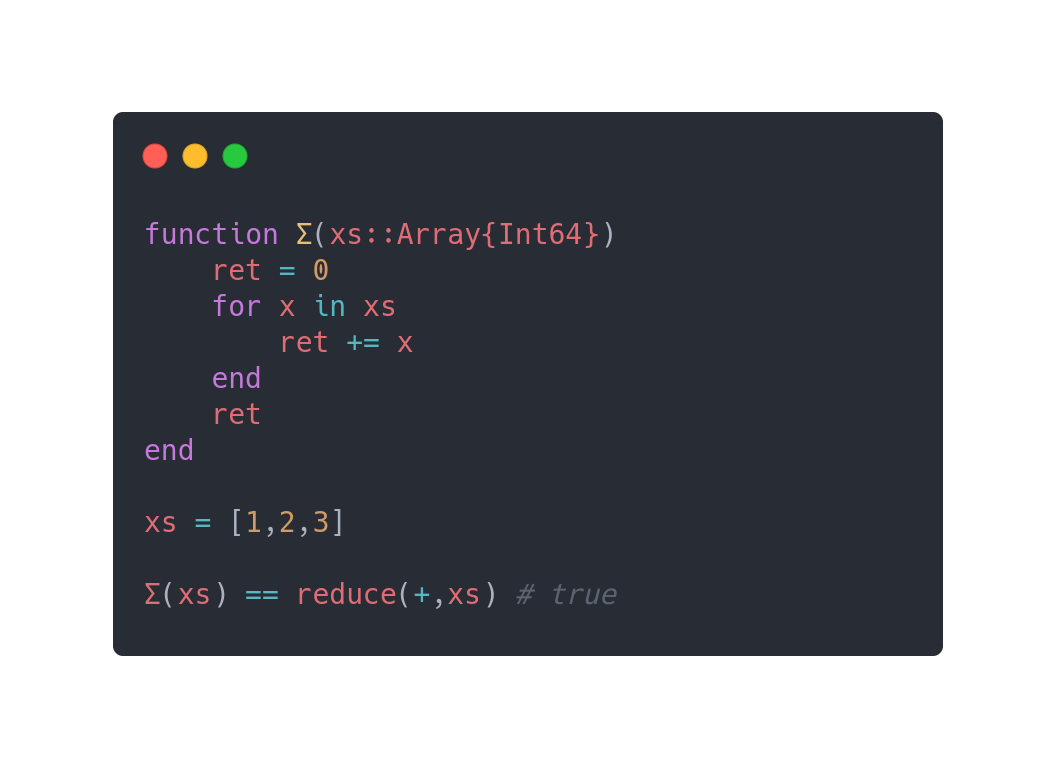
\includegraphics[scale=0.26]{juliaeg.png}
        \caption{Example Julia code}%
        \label{fig:name}
    \end{figure}
\end{frame}

\begin{frame}
Alternative languages include C, Python and Rust
\pause

\textbf{ C:}
\begin{itemize}
    \item Compiles down to binary
    \item Antiquated syntax
    \item Possible (and easy) to write memory unsafe code
    \item Vast array of libraries due to age \& use
    \item No functional properties, harder to implement readable mathematics
\end{itemize}
\pause
\textbf{Python:}
\begin{itemize}
    \item Simple syntax
    \item Wealth of stress-tested libraries
    \item Slow relative to alternatives
    \item unable to compile to binary format
    \item Has some functional capabilities
    \item Has some static typing ability
\end{itemize}
\pause
\end{frame}
\begin{frame}
\textbf{Rust:}
\begin{itemize}
    \item Slower to prototype in as stricter type system to guarantee memory safety
    \item Memory safe, advantage over C/C++
    \item Very performant, runs well on embedded systems
    \item Relatively large binaries due to static dependency linking
    \item Easier to package \& deploy than Julia
\end{itemize}
\end{frame}

\section{Bibliography}
\begin{frame}
\frametitle{References}
\bibliographystyle{abbrv}
\bibliography{lib}
\end{frame}

\end{document}
